\documentclass[border=1pt,tikz]{standalone}

\usepackage{amsmath} % for \dfrac
\usepackage{tikz}
\tikzset{>=latex} % for LaTeX arrow head

\begin{document}


% TIMELINE - particle physics
% sources: http://web.ihep.su/dbserv/compas/src/
%          http://www.particleadventure.org/other/history/
%          https://en.wikipedia.org/wiki/Timeline_of_particle_discoveries
\large
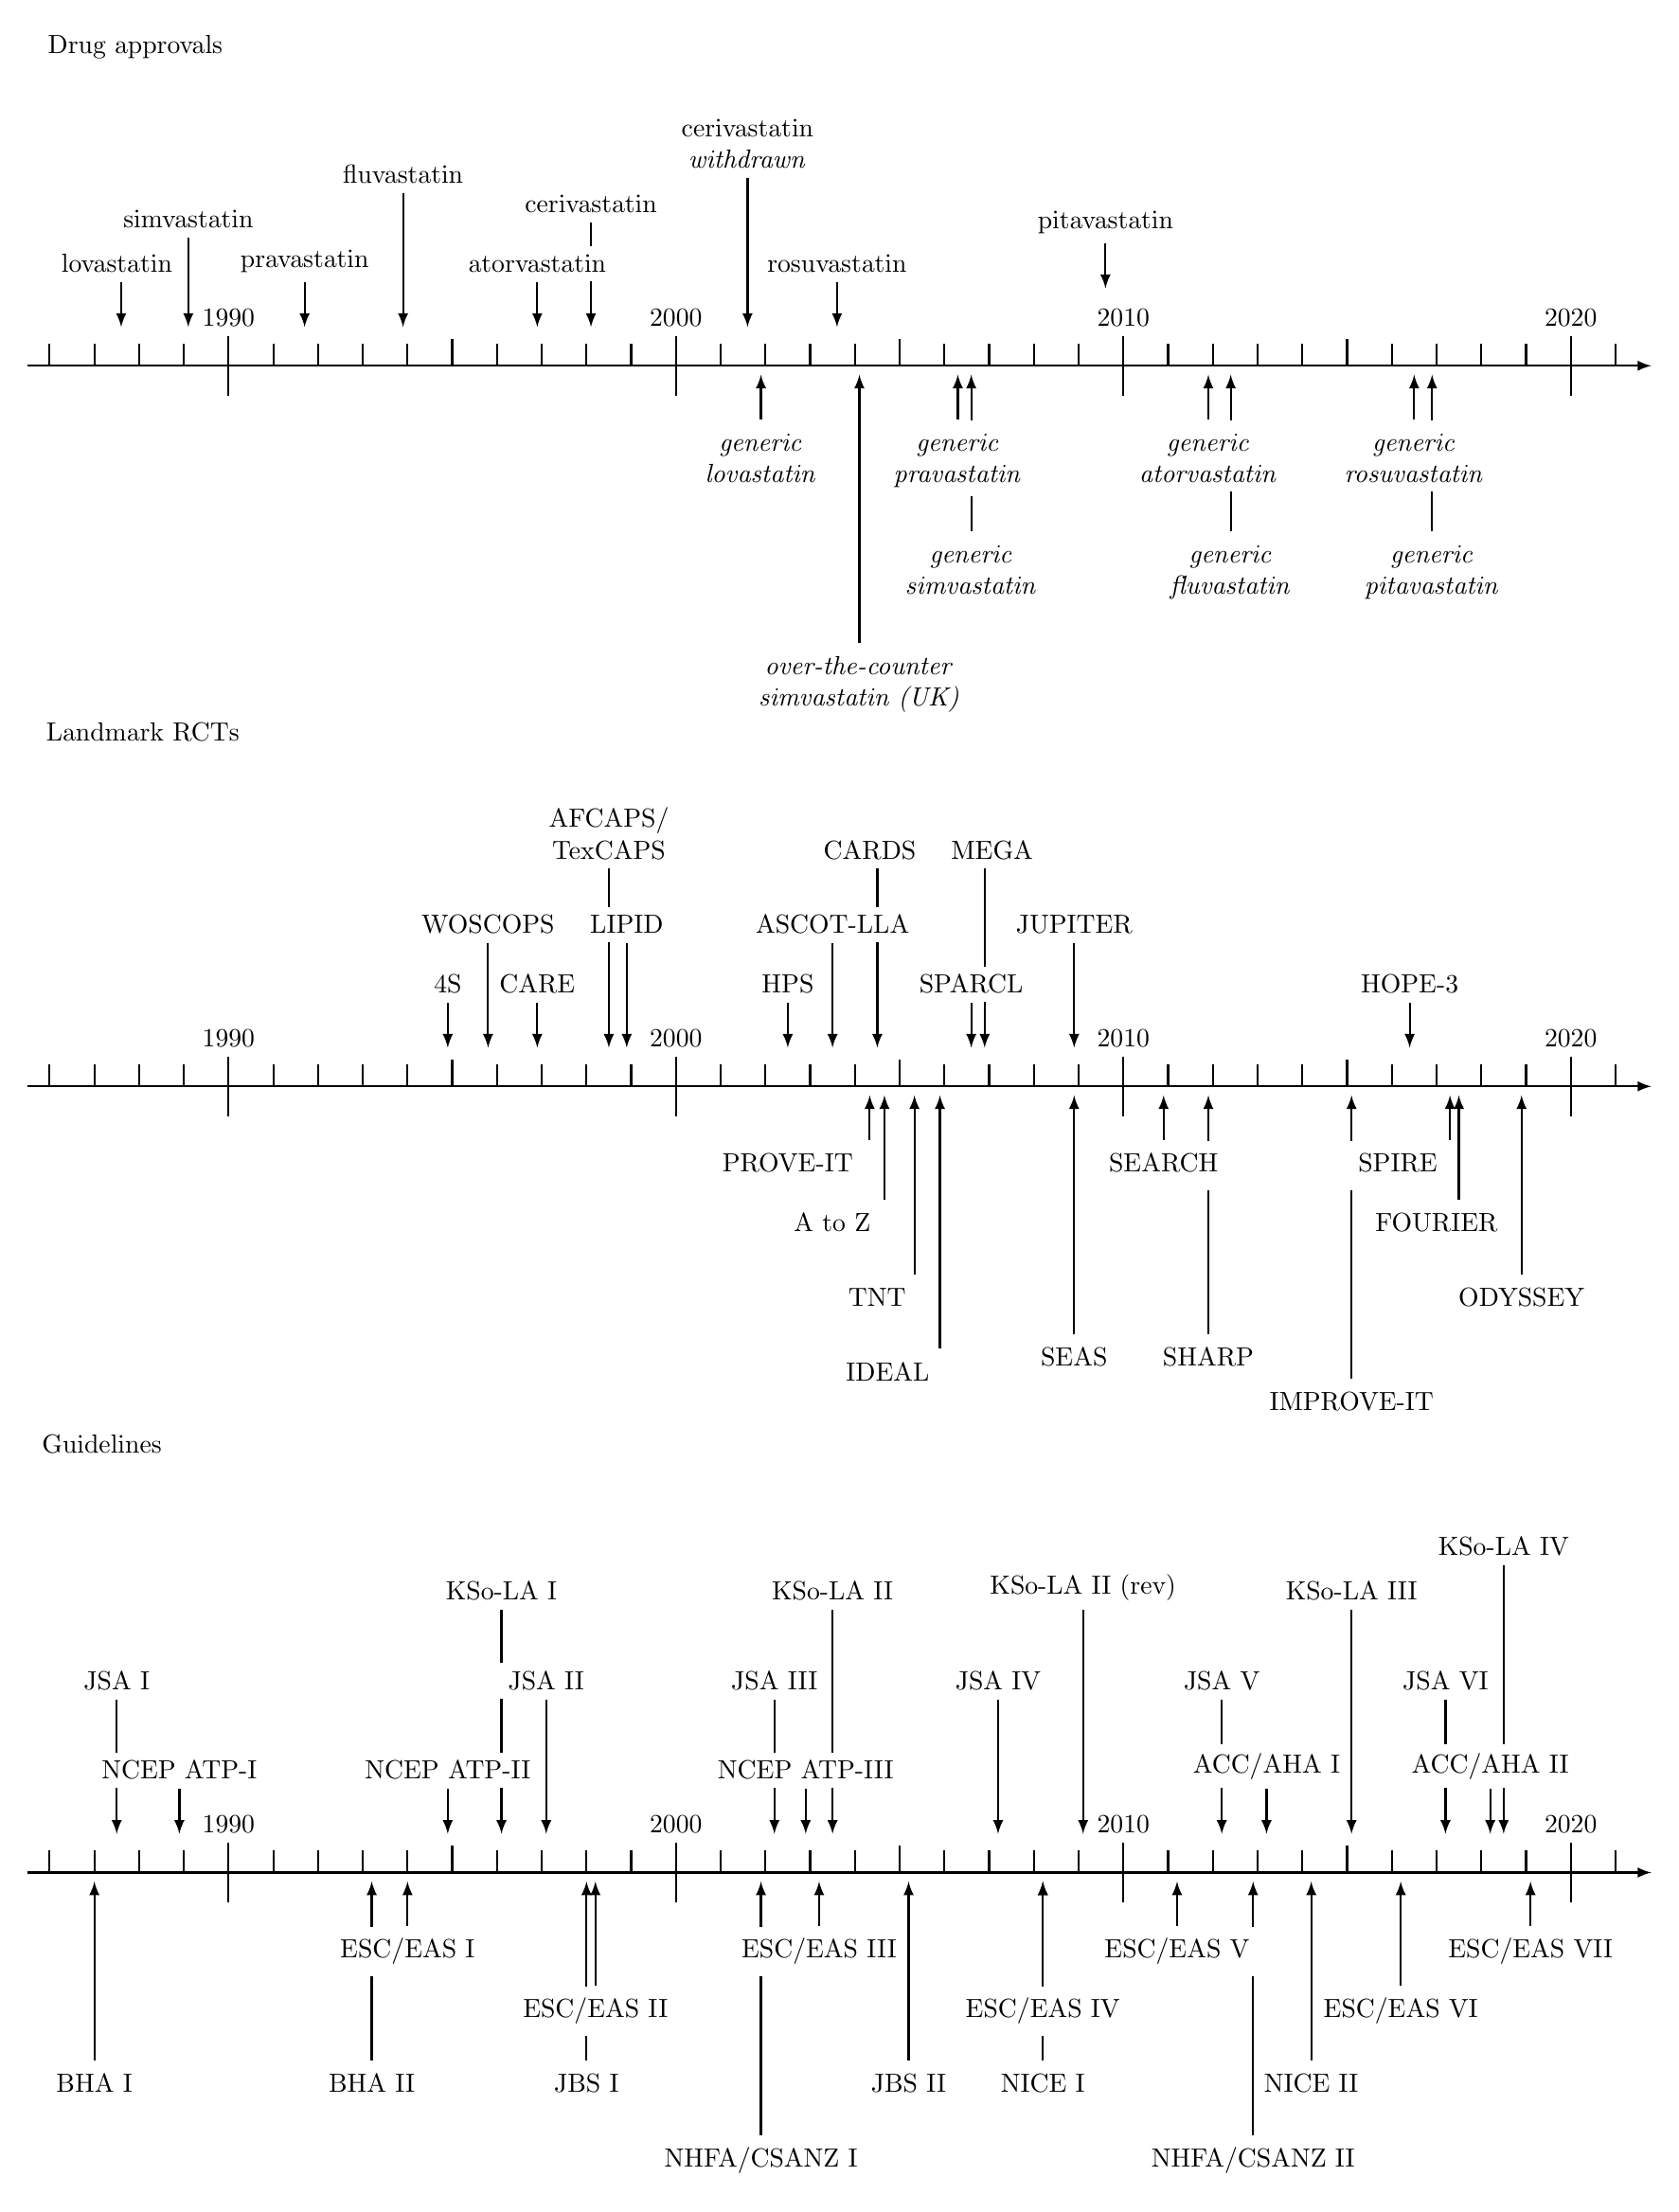
\begin{tikzpicture}[] %[minimum height=10pt, text height=10pt,text depth=10pt,

  % limits
  \newcount\yearOne; \yearOne=1990
  \newcount\yoffset;
  \def\w{18}       % width of axes
  \def\n{3}        % number of decades
  \def\lt{0.40}    %  ten tick length
  \def\lf{0.36}    % five tick length
  \def\lo{0.30}    %  one tick length
  \def\lext{0.15}  % left extension of axes
  \def\rext{1.045} % left extension of axes
  
  % help functions
  \def\yearLabel(#1,#2,#3){\node[above,black!60!blue] at ({(#1-\yearOne)*\w/\n/10},{\lt*#2}) {#3};}
  \def\yearArrowLabel(#1,#2,#3,#4){
    \def\xy{{(#1-\yearOne)*\w/\n/10}}; \pgfmathparse{int(#2*100)};
    \ifnum \pgfmathresult<0 % below
      \def\yyp{{(\lt*(0.90+#2))}}; \def\yyw{{(\yyp-\lt*#3)}}
      \draw[<-,thick,black,align=center]
        (\xy,\yyp) -- (\xy,\yyw)
        node[below] at (\xy,\yyw) {\strut #4};
    \else % under
      \def\yyp{{(\lt*(0.10+#2)}}; \def\yyw{{(\yyp+\lt*#3)}}
      \draw[<-,thick,black,align=center]
        (\xy,\yyp) -- (\xy,\yyw)
        node[above] at (\xy,\yyw) {#4};
    \fi}

    \def\yearArrowLabelBox(#1,#2,#3,#4,#5){
        \def\xy{{(#1-\yearOne)*\w/\n/10}}; \pgfmathparse{int(#2*100)};
        \ifnum \pgfmathresult<0 % below
          \def\yyp{{(\lt*(0.90+#2))}}; \def\yyw{{(\yyp-\lt*#3)}}; \def\xyp{{(\xy - #5)}}
          \draw[<-,thick,black,align=center]
            (\xy,\yyp) -- (\xy,\yyw)
            node[below,black,fill=white] at (\xyp,\yyw) {\strut #4};
        \else % under
          \def\yyp{{(\lt*(0.10+#2)}}; \def\yyw{{(\yyp+\lt*#3)}}; \def\xyp{{(\xy - #5)}}
          \draw[<-,thick,align=center]
            (\xy,\yyp) -- (\xy,\yyw)
            node[above,fill=white] at (\xyp,\yyw) {#4};
        \fi}
  \def\yearArrowLabelRed(#1,#2,#3,#4){
    \def\xy{{(#1-\yearOne)*\w/\n/10}}; \pgfmathparse{int(#2*100)};
      \def\yyp{{(\lt*(0.90+#2))}}; \def\yyw{{(\yyp-\lt*#3)}}
      \fill[red,radius=2pt] (\xy,0) circle;
      \draw[<-,thick,black!25!red,align=center]
        (\xy,\yyp) -- (\xy,\yyw)
        node[below,black!40!red] at (\xy,\yyw) {\strut #4};
     }  
  
  
  %---------------%
  %  1990 - 2020  %
  %---------------%
  
  \yearOne=1990; \advance\yoffset by 130
  \begin{scope}[yshift=-\yoffset]
    
    % axis
    \draw[->,thick] (-\w*\lext,0) -- (\w*1.06,0);
    
    % ticks
    \foreach \tick in {0,1,...,\n}{
      \def\x{{\tick*\w/\n}}
      \def\year{\the\numexpr \yearOne+\tick*10 \relax}
      \draw[thick] (\x,-\lt) -- (\x,\lt) % ten tick
	               node[above] {\year};
      \ifnum \tick<\n
        \draw[thick] ({(\x+\w/\n/2)},0) -- ({(\x+\w/\n/2)},\lf); % five tick
        \foreach \ticko in {1,2,3,4,6,7,8,9}{
          \def\xo{{(\x+\ticko*\w/\n/10)}}
  	      \draw[thick] (\xo,0) -- (\xo,\lo);  % one tick
	  }\fi
    }
    
    % extra ticks
    \draw[thick] (-1*\w/\n/10,0) -- (-1*\w/\n/10,\lo);
    \draw[thick] (-2*\w/\n/10,0) -- (-2*\w/\n/10,\lo);
    \draw[thick] (-3*\w/\n/10,0) -- (-3*\w/\n/10,\lo);
    \draw[thick] (-4*\w/\n/10,0) -- (-4*\w/\n/10,\lo);
    \draw[thick] ({\w+\w/\n/10},0) -- ({\w+\w/\n/10},\lo);
  
    % labels
    % \yearArrowLabel(1980.40,-1.2,1.5,
    %                 $\eta_\text{c}$   )  % 
    % \yearArrowLabel(1981.30,-1.2,1.5,
    %                 B                 )  % 
    % \yearArrowLabel(1983.05,-1.2,1.5,
    %           \mbox{$\text{W}^\pm$\hspace{4pt}}\\
    %                 $\text{D}_\text{s}$\\
    %                 $\Xi_\text{c}$    )  % 
    \yearArrowLabel(1987.6,1.2,1.5,lovastatin ) % 
    \yearArrowLabel(1991.7,1.2,1.5,pravastatin)
    \yearArrowLabel(1989.1,1.2,3,simvastatin)
    \yearArrowLabel(1993.90,1.2,4.5,fluvastatin)  % 
    \yearArrowLabel(1998.10,1.2,3.5,cerivastatin)  %  
    \yearArrowLabelBox(1996.90,1.2,1.5,\mbox{atorvastatin},0)  %
    \yearArrowLabel(2001.60,1.2,5,cerivastatin\\\textit{withdrawn})  %  
    \yearArrowLabel(2003.60,1.2,1.5,rosuvastatin)  % 
    \yearArrowLabel(2009.60,2.5,1.5,pitavastatin)  % 

    \yearArrowLabel(2001.9,-1.2,1.5,\textit{generic}\\\textit{lovastatin}) % 
    \yearArrowLabel(2004.1,-1.2,9,\textit{over-the-counter}\\\textit{simvastatin (UK)}) % 

    \yearArrowLabel(2006.6,-1.2,5.25,\textit{generic}\\\textit{simvastatin}) % 
    \yearArrowLabelBox(2006.3,-1.2,1.5,\textit{generic}\\\textit{pravastatin},0) % 
    \yearArrowLabelBox(2012.4,-1.2,5.25,\textit{generic}\\\textit{fluvastatin},0) % 
    \yearArrowLabelBox(2011.9,-1.2,1.5,\textit{generic}\\\textit{atorvastatin},0) % 
    \yearArrowLabelBox(2016.9,-1.2,5.25,\textit{generic}\\\textit{pitavastatin},0) % 
    \yearArrowLabelBox(2016.5,-1.2,1.5,\textit{generic}\\\textit{rosuvastatin},0) % 

    \node[above,] at (-1.25,4) {Drug approvals};

  \end{scope}

  \yearOne=1990; \advance\yoffset by 275
  \begin{scope}[yshift=-\yoffset]
    
    % axis
    \draw[->,thick] (-\w*\lext,0) -- (\w*1.06,0);
    
    % ticks
    \foreach \tick in {0,1,...,\n}{
      \def\x{{\tick*\w/\n}}
      \def\year{\the\numexpr \yearOne+\tick*10 \relax}
      \draw[thick] (\x,-\lt) -- (\x,\lt) % ten tick
	               node[above] {\year};
      \ifnum \tick<\n
        \draw[thick] ({(\x+\w/\n/2)},0) -- ({(\x+\w/\n/2)},\lf); % five tick
        \foreach \ticko in {1,2,3,4,6,7,8,9}{
          \def\xo{{(\x+\ticko*\w/\n/10)}}
  	      \draw[thick] (\xo,0) -- (\xo,\lo);  % one tick
	  }\fi
    }
    
    % extra ticks
    \draw[thick] (-1*\w/\n/10,0) -- (-1*\w/\n/10,\lo);
    \draw[thick] (-2*\w/\n/10,0) -- (-2*\w/\n/10,\lo);
    \draw[thick] (-3*\w/\n/10,0) -- (-3*\w/\n/10,\lo);
    \draw[thick] (-4*\w/\n/10,0) -- (-4*\w/\n/10,\lo);
    \draw[thick] ({\w+\w/\n/10},0) -- ({\w+\w/\n/10},\lo);
  
    % labels
    \yearArrowLabel(1994.9,1.2,1.5,4S) 
    \yearArrowLabel(1995.8,1.2,3.5,WOSCOPS) 
    \yearArrowLabel(1998.5,1.2,6,AFCAPS/\\TexCAPS) 

    \yearArrowLabel(2008.9,-1.2,8,SEAS)  % 
    \yearArrowLabel(2011.9,-1.2,8,SHARP)  % 
    \yearArrowLabel(2015.1,-1.2,9.5,IMPROVE-IT) 

    \yearArrowLabel(1996.9,1.2,1.5,CARE) 
    \yearArrowLabelBox(1998.9,1.2,3.5,LIPID,0) 
    \yearArrowLabelBox(2010.9,-1.2,1.5,SEARCH,0)  % 
    \yearArrowLabelBox(2008.9,1.2,3.5,JUPITER,0)  % 
    \yearArrowLabelBox(2005.9,-1.2,8.5,IDEAL,0.7)  % 
    \yearArrowLabelBox(2005.33,-1.2,6,TNT,0.5)  %
    \yearArrowLabelBox(2004.66,-1.2,3.5,A to Z,0.7)  % 
    \yearArrowLabelBox(2004.33,-1.2,1.5,PROVE-IT,1.1)  % 
    \yearArrowLabelBox(2002.5, 1.2,1.5,HPS,0)   %  
    \yearArrowLabelBox(2006.9,1.2,6,MEGA,-0.1)  % 
    \yearArrowLabelBox(2006.6,1.2,1.5,SPARCL,0)  % 

    \yearArrowLabelBox(2004.5,1.2,6,CARDS,0.1)  % 
    \yearArrowLabelBox(2003.5,1.2,3.5,ASCOT-LLA,0)  % 

   % 
    \yearArrowLabel(2016.4,1.2,1.5,HOPE-3)  % 

    \yearArrowLabelBox(2018.9,-1.2,6,ODYSSEY,0)  % 
    \yearArrowLabelBox(2017.5,-1.2,3.5,FOURIER,0.3)  % 
    \yearArrowLabelBox(2017.3,-1.2,1.5,SPIRE,0.7)  % 

    %\yearArrowLabelRed(2017.7,-1.2,1.5,X\\\,$\text{B}'$) % low mass
    %\yearArrowLabelRed(2020.9,-1.2,1.5,LQ) % leptoquark
    
    \node[below] at (-1.15,5) {Landmark RCTs};

  \end{scope}
  
  \yearOne=1990; \advance\yoffset by 300
  \begin{scope}[yshift=-\yoffset]
    
    % axis
    \draw[->,thick] (-\w*\lext,0) -- (\w*1.06,0);
    
    % ticks
    \foreach \tick in {0,1,...,\n}{
      \def\x{{\tick*\w/\n}}
      \def\year{\the\numexpr \yearOne+\tick*10 \relax}
      \draw[thick] (\x,-\lt) -- (\x,\lt) % ten tick
	               node[above] {\year};
      \ifnum \tick<\n
        \draw[thick] ({(\x+\w/\n/2)},0) -- ({(\x+\w/\n/2)},\lf); % five tick
        \foreach \ticko in {1,2,3,4,6,7,8,9}{
          \def\xo{{(\x+\ticko*\w/\n/10)}}
  	      \draw[thick] (\xo,0) -- (\xo,\lo);  % one tick
	  }\fi
    }
    
    % extra ticks
    \draw[thick] (-1*\w/\n/10,0) -- (-1*\w/\n/10,\lo);
    \draw[thick] (-2*\w/\n/10,0) -- (-2*\w/\n/10,\lo);
    \draw[thick] (-3*\w/\n/10,0) -- (-3*\w/\n/10,\lo);
    \draw[thick] (-4*\w/\n/10,0) -- (-4*\w/\n/10,\lo);
    \draw[thick] ({\w+\w/\n/10},0) -- ({\w+\w/\n/10},\lo);
  
    % labels

    \yearArrowLabelBox(1996.1,1.2,7.5,KSo-LA I,0) 
    \yearArrowLabelBox(2003.5,1.2,7.5,KSo-LA II,0) 
    \yearArrowLabelBox(2009.1,1.2,7.5,KSo-LA II (rev),0) 
    \yearArrowLabelBox(2015.1,1.2,7.5,KSo-LA III,0) 
    \yearArrowLabelBox(2018.5,1.2,9,KSo-LA IV,0) 
 
    \yearArrowLabelBox(1987.5,1.2,4.5,JSA I,0) 
    \yearArrowLabelBox(1997.1,1.2,4.5,JSA II,0) 
    \yearArrowLabelBox(2002.2,1.2,4.5,JSA III,0) 
    \yearArrowLabelBox(2007.2,1.2,4.5,JSA IV,0) 
    \yearArrowLabelBox(2012.2,1.2,4.5,JSA V,0) 
    \yearArrowLabelBox(2017.2,1.2,4.5,JSA VI,0) 
    
    \yearArrowLabelBox(1988.9,1.2,1.5,NCEP ATP-I,0) 
    \yearArrowLabelBox(1994.9,1.2,1.5,NCEP ATP-II,0) 
    \yearArrowLabelBox(2002.9,1.2,1.5,NCEP ATP-III,0) 
    \yearArrowLabelBox(2013.2,1.2,1.5,ACC/AHA I,0) 
    \yearArrowLabelBox(2018.2,1.2,1.5,ACC/AHA II,0) 


    \yearArrowLabel(2001.9,-1.2,8.5,NHFA/CSANZ I) 
    \yearArrowLabel(2012.9,-1.2,8.5,NHFA/CSANZ II)
    \yearArrowLabelBox(1987,-1.2,6,BHA I,0) 
    \yearArrowLabelBox(1993.2,-1.2,6,BHA II,0) 
    \yearArrowLabelBox(1998,-1.2,6,JBS I,0) 
    \yearArrowLabelBox(2005.2,-1.2,6,JBS II, 0) 
    \yearArrowLabelBox(2008.2,-1.2,6,NICE I,0) 
    \yearArrowLabelBox(2014.2,-1.2,6,NICE II,0) 
    \yearArrowLabelBox(1994,-1.2,1.5,ESC/EAS I,0) 
    \yearArrowLabelBox(1998.2,-1.2,3.5,ESC/EAS II,0) 
    \yearArrowLabelBox(2003.2,-1.2,1.5,ESC/EAS III,0) 
    \yearArrowLabelBox(2008.2,-1.2,3.5,ESC/EAS IV,0) 
    \yearArrowLabelBox(2011.2,-1.2,1.5,ESC/EAS V,0) 
    \yearArrowLabelBox(2016.2,-1.2,3.5,ESC/EAS VI,0) 
    \yearArrowLabelBox(2019.1,-1.2,1.5,ESC/EAS VII,0) 

    
    %\yearArrowLabelRed(2017.7,-1.2,1.5,X\\\,$\text{B}'$) % low mass
    %\yearArrowLabelRed(2020.9,-1.2,1.5,LQ) % leptoquark
    
    \node[below] at (-1.7,6) {Guidelines};

  \end{scope}
  
\end{tikzpicture}



\end{document}